\section{Working on XSTAMPP}

\subsection{Setting up the environment}
\begin{itemize}
\item \href{http://eclipse.org/downloads}{Eclipse for RCP and RAP Developers (Plug-in Developement)}\footnote{\url{http://eclipse.org/downloads}} ($> Lunar$)
\item At least JavaSE 1.7
\item To install gef ( \textit{help}$\rightarrow$\textit{install new software}$\rightarrow$\textit{http://download.eclipse.org/tools/gef/updates/releases/})
\item To install nebula grid from eclipse.org\footnote{\url{http://download.eclipse.org/technology/nebula/snapshot/}}
\item To install maven\footnote{\url{https://maven.apache.org/download.cgi}}
\item import/clone xstampp projects using the included git
	\begin{enumerate}
	\item open the \textit{Import} Dialog selecting \textit{File}$\rightarrow$\textit{Import}
	\item in the Import menu click \textit{Git}$\rightarrow$\textit{Projects from Git} and follow the steps of the import wizard
	\end{enumerate}
\item To resolve upcoming error messages refer to Known Issues Section \ref{chap:issues}
\end{itemize}

\subsection{Running XSTAMPP from Eclipse}
\begin{enumerate}
\item Go to \textit{xstampp.repository}$\rightarrow$\textit{xstampp.product}
\item In the product editor click on  \textit{Testing}$\rightarrow$ \textit{Launch an Eclipse Application}
\item The run fails on the first try, which is normal because we haven't included the required plugins yet
\item In the last step Eclipse has created a \textit{Run configuration} for us which we are going to use now
	\begin{enumerate}
	\item right click on the \textit{xstampp} project and select \textit{Run As}$\rightarrow$ \textit{Run Configurations..}
	\item in the opening dialog search for the Plug-ins Tab (see figure \ref{fig:runConfig})(you may need to adjust the size of the window)
	\item you can now include/exclude the xstampp plug-ins included in your runtime
	\item finally find/press the button \textit{Add Required Plug-ins} and Apply/Run the run configuration
	\end{enumerate}
\end{enumerate}
\begin{figure}[H]
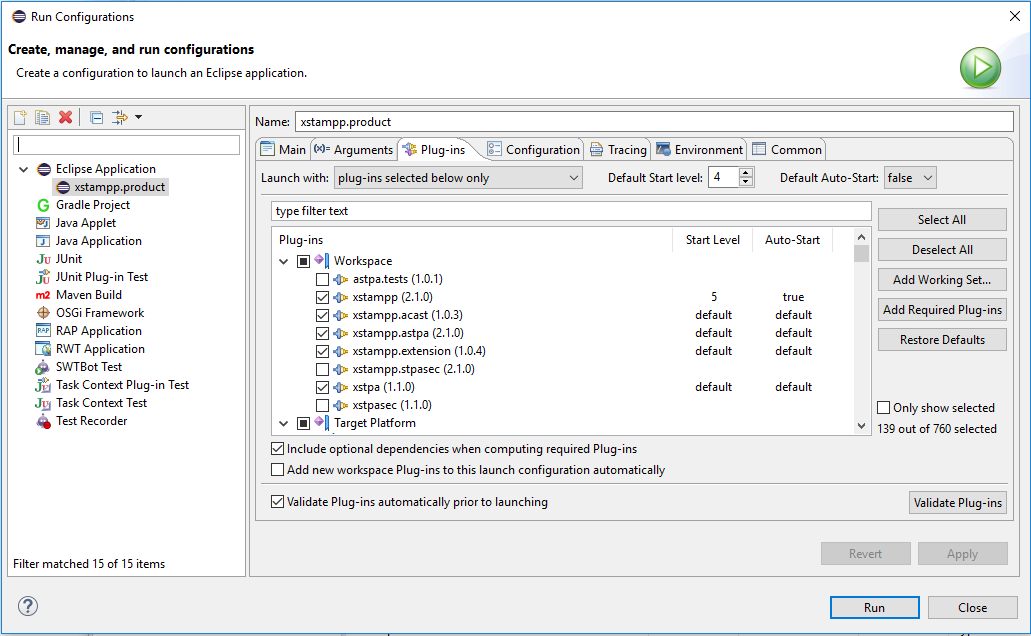
\includegraphics[scale=0.5]{images/runConfig.png}
\caption{Before eclipse can successfully run xstampp the required plug-ins must be included in the runtime}
\label{fig:runConfig}
\end{figure}

\subsection{Contribute}
\begin{itemize}
\item Setting up Eclipse Preferences (open \textit{Eclipse}$\rightarrow$\textit{Window}$\rightarrow$\textit{Preferences}):
\begin{enumerate}
	\item Go to \textit{XML}$\rightarrow$\textit{XML Files}$\rightarrow$\textit{Editor}
	\begin{enumerate}
		\item set the \textit{Line width} to \textbf{120}
		\item check the radio box \textit{Indent using spaces}
		\item set \textit{Indentation size} to \textbf{4}
	\end{enumerate}
	\item Go to \textit{Java}$\rightarrow$\textit{Code Style}$\rightarrow$\textit{Formatter}
	\begin{enumerate}
		\item Press \textit{Import...}
		\item Import the $java\_formatter.xml$ in $<repo>$\textit{/xstampp/misc/java}$\_$\textit{formatter.xml}
	\end{enumerate}
\end{enumerate}
\end{itemize}
\subsubsection{Create a new plugin:}
\begin{itemize}
\item Contributing plugins should be named as \textit{xstampp.}$<your Plugin>$
\item Create a new plugin by clicking \textit{New}$\rightarrow$\textit{Others..}$\rightarrow$\textit{Plug-in Developement}$\rightarrow$\textit{Plug-in Project}
\item Add dependencies xstampp and xstampp.extension
\item Add the extension xstampp.extension.steppedProcess to your plugin
\item Create a class implementing IDataModel
\item Create stepEditors which must extend StandartEditorPart and implement IViewBase
\item Xstampp loads the files which are selected in the load Dialog or already located in the workspace 
	  by directly calling a load command registered as command in the steppedProcess extensionPoint herefore it needs:
	\begin{itemize}
	\item a load job which extends AbstractLoadJob
	\item a load Handler extending AbstractHandler which is registered as default handler for the load command 
	\item let your handler.execute() return a new instance of your load job
	\end{itemize}
\item XSTAMPP uses Eclipse Tycho as build tool, to include a  plugin into its build process it need to be configured as Maven plugin\footnote{\url{http://www.vogella.com/tutorials/EclipseTycho/article.html}}
\end{itemize}

\subsubsection{Create a new Version} 
\begin{itemize}
\item All changes must be recorded in the $CHANGELOG.md$
\item If \textit{misc/docu/README.tex} has been changed than:
	\begin{itemize}
	\item Download LaTex(\href{https://miktex.org/}{MikTex}\footnote{https://miktex.org/} for Windows or \href{http://tug.org/mactex/}{MacTex}\footnote{http://tug.org/mactex/} for Mac)
	\item This should contain an html(for eclipse help), md(for GitHub) and a pdf version of the Readme this can be achived by using \href{https://pandoc.org}{Pandoc}\footnote{https://pandoc.org}
		\begin{itemize}
		\item \texttt{cd misc/docu}
		\item \texttt{pandoc -s README.tex -o README.pdf --toc}
		\item \texttt{pandoc -s README.tex -o README.html}
		\item \texttt{pandoc -s README.tex -o README.md}
		\item \texttt{cp README.html ../../README/html/}
		\item \texttt{cp README.pdf ../../}
		\end{itemize}
	\end{itemize}
\item Update the \textit{xstampp/html/CHANGELOG.html} (using Pandoc):
	\begin{itemize}
		\item \texttt{cd ../..}
		\item \texttt{pandoc -s CHANGELOG.md -o CHANGELOG.html}
		\item \texttt{cp CHANGELOG.html xstampp/html/}
	\end{itemize}
	\item \textit{createFiles.cmd} is a Windows batch script that executes all of the above commands to create the release files
\end{itemize}